\fig{fv:e2:slip}{摩擦反向交换动量，相对速度图的面积决定是否滑出木板}{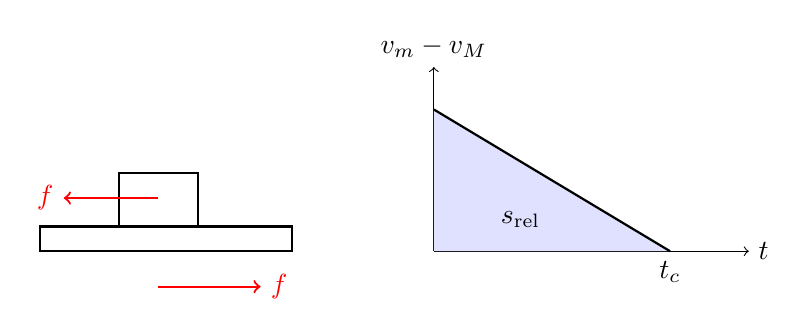
\begin{tikzpicture}[x=1cm,y=.9cm]
\draw[thick](0,0)rectangle(3.2,.35);\draw[thick](1,.35)rectangle(2,1.1);
\draw[->,red,thick](1.5,.75)--(.3,.75)node[left]{$f$};\draw[->,red,thick](1.5,-.5)--(2.8,-.5)node[right]{$f$};
\begin{scope}[xshift=5cm]\draw[->](0,0)--(4,0)node[right]{$t$};\draw[->](0,0)--(0,2.6)node[above]{$v_m-v_M$};
\fill[blue!12](0,0)--(0,2)--(3,0)--cycle;\draw[thick](0,2)--(3,0);\node[below]at(3,0){$t_c$};\node at(1.1,.45){$s_{\rm rel}$};\end{scope}
\end{tikzpicture}}
图\ref{fv:e2:slip}左侧两摩擦力属于不同物体，所以在整体动量式中相消，在各自方程中却都要保留。右侧画的是相对速度，蓝色面积 $s_{\rm rel}=\int_0^{t_c}(v_m-v_M)\dd t$才是物块在板上走过的长度。对地位移中还包含板的运动，不能直接拿它与板长比较。若板端先被到达，共速条件尚未实现，便须提前结束这段摩擦模型。
